\documentclass[10pt]{article}

\usepackage{amsmath}
\usepackage{fullpage}
\usepackage{array}
\usepackage{graphicx}
\usepackage{gensymb}
\usepackage{booktabs}
\usepackage{gensymb}
\usepackage{graphicx}

\graphicspath{ {../Images/} }

\date{2014-6-22}
\pagestyle{empty}
\setlength{\parindent}{0pt}

\begin{document}
\begin{center}
\begin{Large}\textbf{Chapter: Frictional Force}\end{Large} \\
\smallskip
%\begin{large} Acceleration \end{large}
\end{center}
%%%%%%%
Objectives: Distinguish between static and kinetic friction, determine the direction and magnitude of frictional force.
\section{Frictional Force}
Definition: The tendency of a surface to oppose the \emph{relative} motion is called friction and the associated force is known as the frictional force. 

Consider a book kept on the table at rest.  Now we apply very small force parallel to the surface of the table.  The book doesn't move because there is a friction between the surface of the book and that of table which tend to oppose the relative motion.  We increase the magnitude of the applied force and the book still doesn't move.  This means that the frictional force also increased (why?). Now we apply force with larger magnitude and then the book starts moving on the surface of the table.  There is still frictional force but it is smaller than the applied force.  The graph of this process is as following      
\begin{figure}[h]
\label{skfriction}
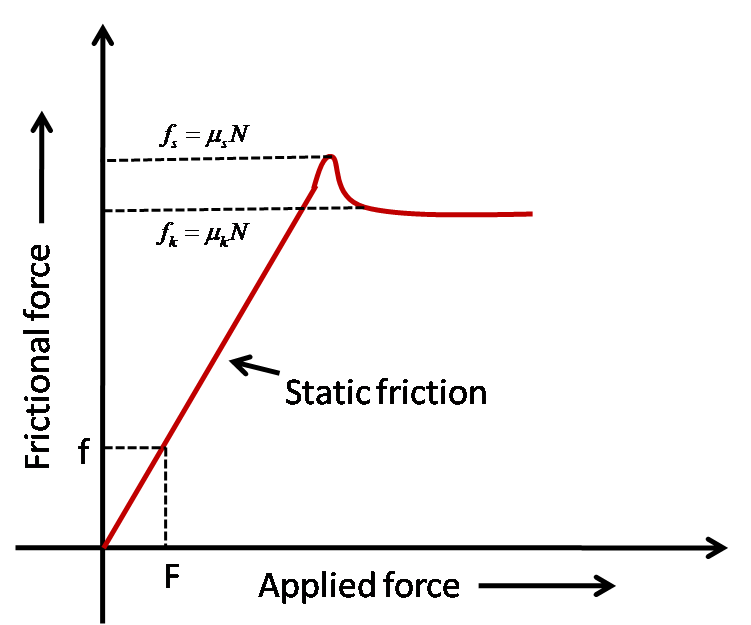
\includegraphics[scale=.5]{static_fric}
\centering
\caption{Frictional force vs applied force}
\centering
\end{figure}

\subsection{Types of friction}
There are two types of frictional forces: 
\begin{enumerate}
\item Static friction is  the frictional force for body at rest.  The magnitude is given by
  \begin{equation}
    f_s=\mu_sN
  \end{equation}
where $N$ is the normal or contact force and $\mu_s$ is the coefficient of static friction.
\item Kinetic friction is the frictional force for body in motion. The magnitude is given by
  \begin{equation}
    f_k=\mu_kN
  \end{equation}
where $\mu_k$ is the coefficient of kinetic friction.
\end{enumerate}

In the figure \ref{skfriction}, the linear part corresponds to the static friction. It shows that the static frictional force is directly proportional to the applied force.  The latter part corresponds to the kinetic friction.

The maximum value of the static friction is always greater than the kinetic friction.  This implies that $\mu_s>\mu_k$

\end{document}
